% !TeX root = ../../../thesis.tex

\section{Simulation}
\label{sec:simulation-evaluation}

In \autoref{sec:hardware-evaluation} the evaluation of the hardware and software was shown using the continuous transmission method, as detailed in \autoref{subsec:continuous-method-modulation}.
Since this is already been evaluated and proven, in this simulation section the scalability of a larger system will be evaluated, using the probabilistic method as explained in \autoref{subsec:probabilistic-method-modulation}.


Before the actual simulation itself, parameters such as $\epsilon$ need to be set.
1 - $\epsilon$, is the probability that for every point in time the number of LEDs that are modulating will not exceed $m$, as discussed in \autoref{subsec:probabilistic-method-modulation}.
This will determine if interference can occur and therefor the overall accuracy and correctness of the system.

For the rest of this simulation a Gold sequence set with length 127 will be used for the assessment.
This set has 129 unique Gold sequences.

This simulation does the following: 

\begin{itemize}

	\item For the set values of the sequence set, $\epsilon$ and $\epsilon_1$, the probability $p$ and the time to complete the $k$ attemtps are calculated (See \autoref{subsec:probabilistic-method-modulation}).

	\item For each attempt, from the total $k$ runs, it is decided which transmitters will transmit. The probability $p$ is used for this. $k$ depends on $p$ and $\epsilon_1$.

	\item If a certain transmitter is selected to transmit, its code sequence is added to a signal vector. One particular transmitter may be not selected at all, or many times, again probability $p$ is used for this.

	\item When the entire signal has been constructed, the decoding process begins. All sequences in the set are used to decode the incoming signal for every time step.

	\item During the decoding, the results are analyzed and together with the information that is known when a particular transmitter transmitted at what time, the results are classified into four categories: true-positive, true-negative, false-positive and false-negative. This is done for each point in time.

	\item With those four categories, the precision, recall and the F-measure are calculated.



\end{itemize}




Let's set $\epsilon = 0.1$, meaning that the probability that there will be less than or equal to $m$ LEDs modulating for every point in time will be 0.9 or 90 \%, where $m$ is the maximum number of simultaneous transmitters such that no destructive interference takes place.
Let's also set $\epsilon_1 = \epsilon = 0.1$, meaning the probability that all LEDs will have modulated at least once is equal to 0.9 or 90 \%.
The Gold sequence with length 127 has 129 unique sequences.
With these values and the Gold sequence set, the simulation as described above can begin. 



The results of the simulation can be seen in \autoref{fig:sim-concurrent-tx-and-f-measure-eps=1-n=7}.
In this figure the number of concurrent transmitters can be seen. 
The maximum number of simultaneous transmitters such that no destructive interference takes place, $m$, is also visible here.
When the number of concurrent transmitters is below or equal to the $m$-line, it is guarantied that no interference will occur, as proven in \autoref{sec:interference-solution}.
But when the number of concurrent transmitters is above the $m$-line, it is possible that there will be interference but it is not always the case.
This depends on what the cross correlation with the other sequences is and if they cancel each other out or if they enhance each other.
Also in \autoref{fig:sim-concurrent-tx-and-f-measure-eps=1-n=7}, it can be seen that whenever the number of concurrent transmitters is below the $m$-line, the F-measure is equal to 1.
This means that everything in the decoding process went well, no false-positives and/or false-negatives.
When the number of concurrent transmitters is above the $m$-line, two things can happen: either there is enough interference to cause false-positives and/or false-negatives, or there is not enough interference and everything will go well.
Multiple times the number of concurrent transmitters is so high, it causes interference as can be seen in the F-measure, which has drops at the same time as when the number of concurrent transmitters is too high.
In \autoref{fig:sim-concurrent-tx-and-f-measure-eps=1-n=7} the percentage of transmitters that have transmitted at least once can also be seen.
After the $k$ attempts are simulated, the part of the transmitters that actually transmitted at least once is roughly 90 \%.
Which is the expected value when $\epsilon_1 = 0.1$.
$1 - \epsilon_1$ is the probability that a transmitter will have transmitted at least once after $k$ attempts.
Since all transmitters are independent and identically distributed, this probability holds for all transmitters.
Also the percentage that the number of concurrent transmitters is above $m$ is roughly equal to 8 \%.
This number will get closer and closer to $\epsilon_1$ the longer the simulation takes.





\begin{figure}[tbp]
	\centering
	\includegraphics[width=\textwidth]{chapters/evaluation-chapters/simulation/sim-concurrent-tx-and-f-measure-eps=1-n=7.eps}
	\caption{Results of the simulation. Figure shows the number of concurrent transmitters at each point in time along with $m$ and the percentage of transmitters that have transmitted at least once. Also the F-measure is shown.}
	\label{fig:sim-concurrent-tx-and-f-measure-eps=1-n=7}
\end{figure}









The time that the simulation takes is roughly 2.2 s.
The time corresponds with the theoretical time calculated in \autoref{subsec:probabilistic-method-modulation} as can be seen in \autoref{tbl:probabilistic-method-time-as-function-N}.
So this was a fast time and pretty accurate, considering that there were only a few drops in the F-measure.
But roughly 10 \% of the transmitters did not even transmit once.










The same simulation is done again, but now with $\epsilon = \epsilon_1 = 0.001$.
The plots can be seen in \autoref{fig:sim-concurrent-tx-and-f-measure-eps=001-n=7}.
Note that all transmitters have transmitted at least once.
%A couple of times the number of concurrent transmitters goes above the $m$-line, but it does not cause interference as shown be the F-measure, which is a constant 1.
At no time the number of concurrent transmitters goes above the $m$-line, so there will be no interference as can also be seen by looking at the F-measure which is a constant 1.
So with $\epsilon = \epsilon_1 = 0.001$ it is an accurate setup that can use all the sequences in the set.
But the simulation takes roughly 25 s.
The time corresponds with the theoretical time calculated in \autoref{subsec:probabilistic-method-modulation} as can be seen in \autoref{tbl:probabilistic-method-time-as-function-N}.
This is still a relative small amount of time, but still 10 times larger than the previous simulation.


\begin{figure}[tbp]
	\centering
	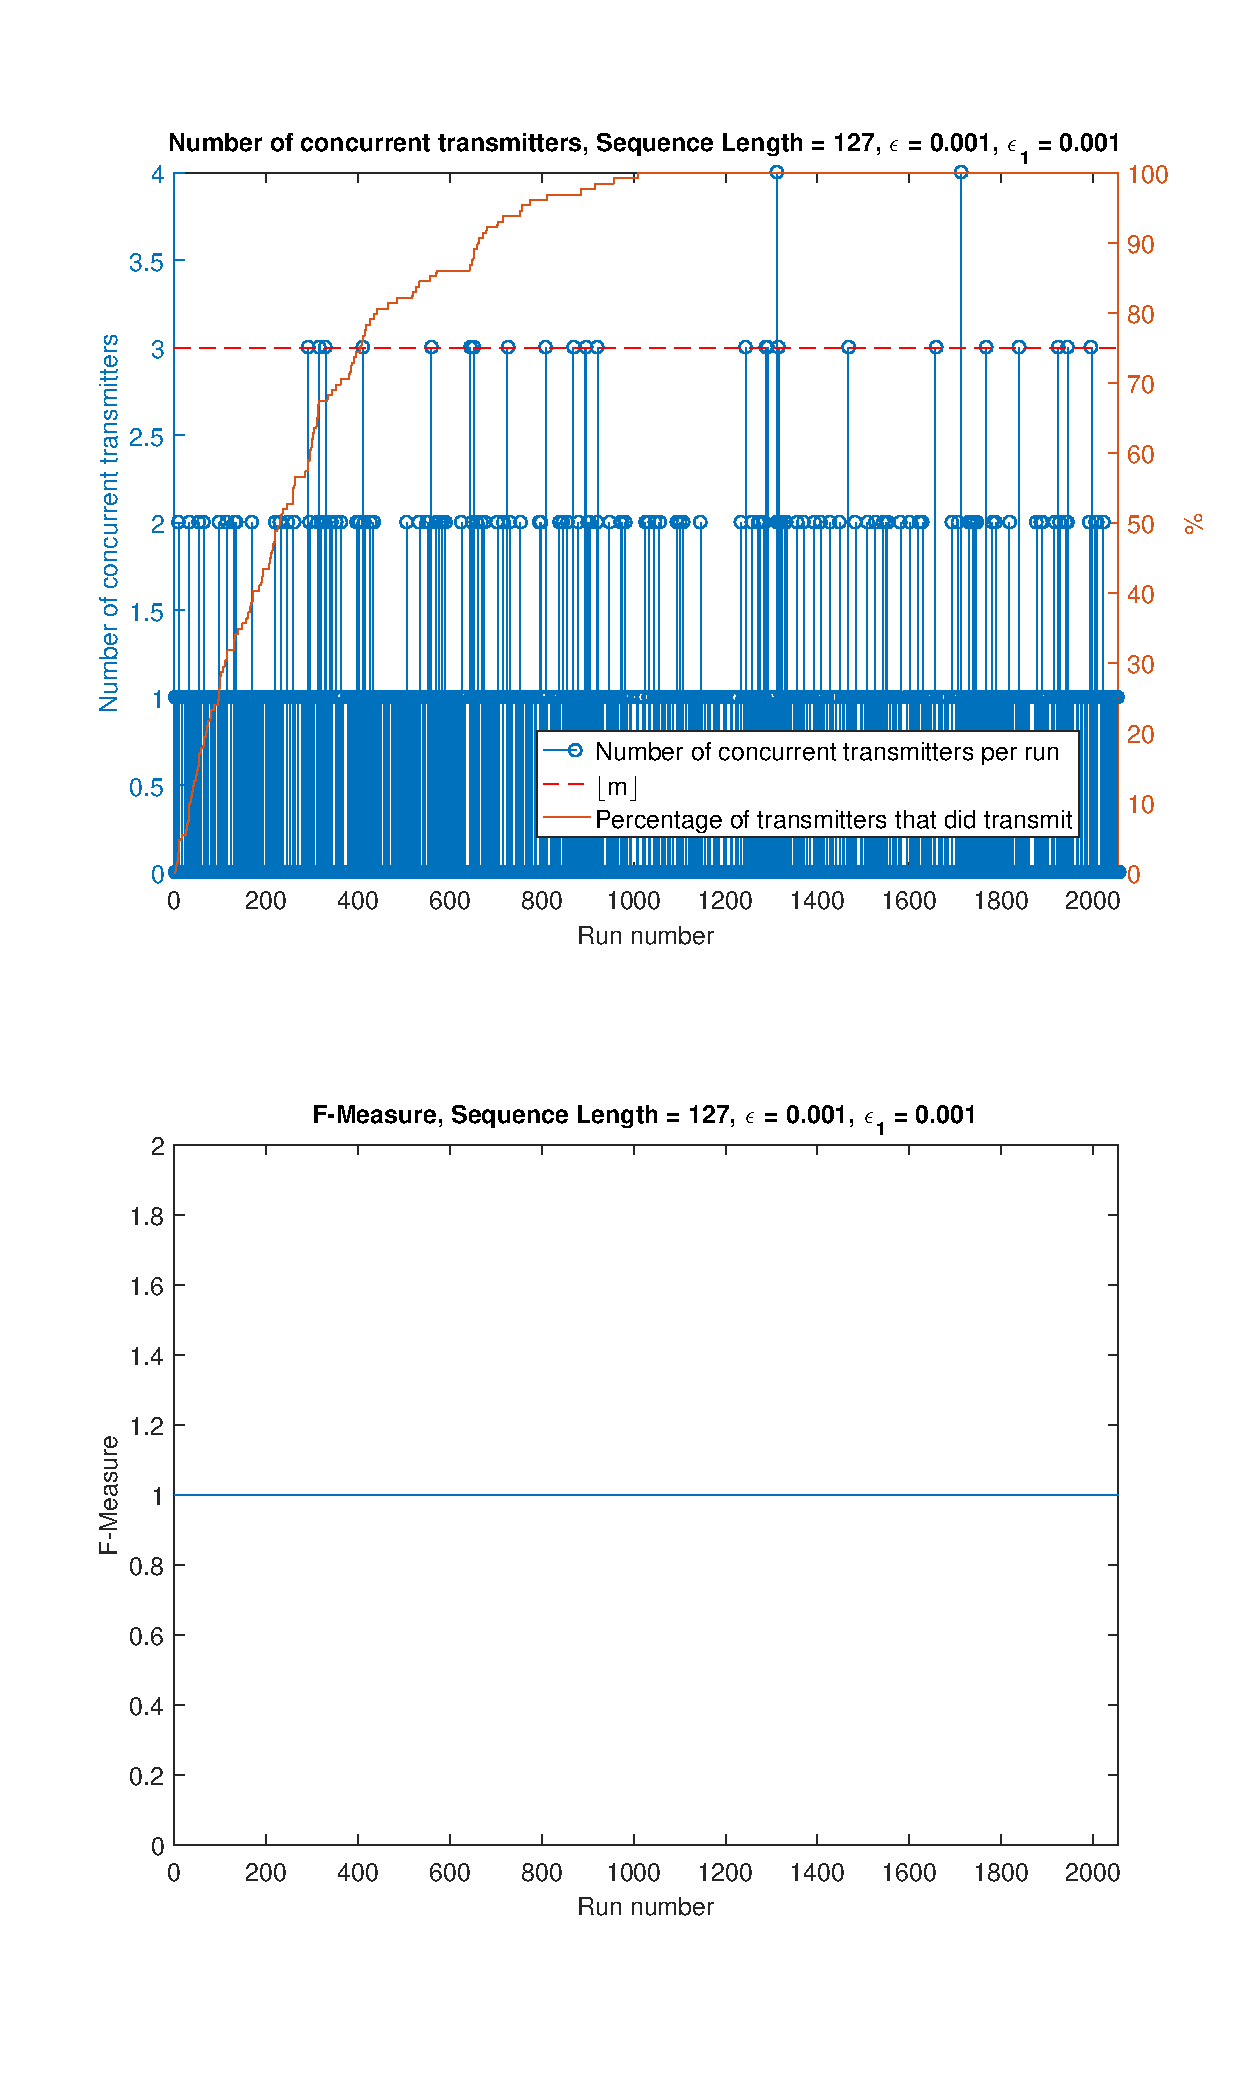
\includegraphics[width=\textwidth]{chapters/evaluation-chapters/simulation/sim-concurrent-tx-and-f-measure-eps=001-n=7.eps}
	\caption{Results of the simulation. Upper plot shows the number of concurrent transmitters per run along with $m$. The lower plot shows the F-measure per run.}
	\label{fig:sim-concurrent-tx-and-f-measure-eps=001-n=7}
\end{figure}

 

These simulations show that for the probabilistic method there is a clear trade off between time and accuracy.
For a given set of sequences, a low value for $\epsilon$ gives high accuracy but the also the a high time.
A high value for $\epsilon$ gives lower accuracy but the also the time becomes smaller.
A low value for $\epsilon_1$ yields a high completeness, in terms of transmitters that have transmitted, for the simulation but also makes the time grow larger.
A simulation with a high value for $\epsilon_1$ will have a low completeness but is also done more quickly.